\section*{سوال ۳}

\begin{enumerate}[label=\alph*)]

\item 
شکل زیر را در نظر بگیرید:  

\begin{figure}[H]
    \centering
    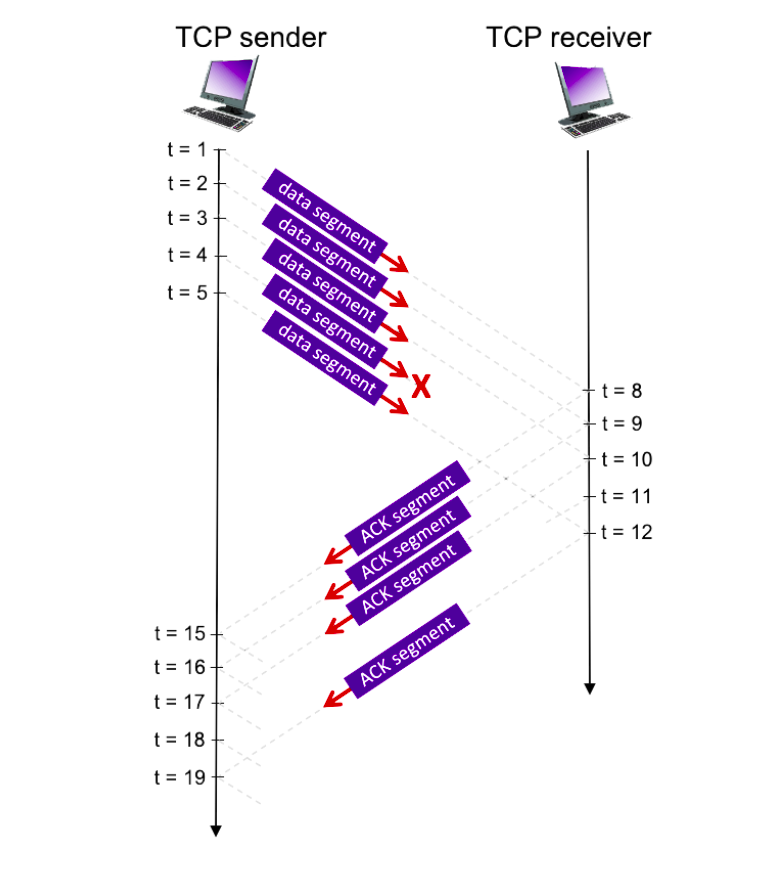
\includegraphics[width=0.95\textwidth]{Questions/pics/Q3.png}
    \caption{}
    \label{fig:small-example}
\end{figure}

فرض کنید مقدار \lr{Sequence Number} در ابتدا برابر با ۱۶۶ است و هر سگمنت دارای ۱۹۹ بایت داده می‌باشد.  
مقدار \lr{ACK} و \lr{Sequence Number} را برای تمامی پکت‌ها بنویسید.

\item 
فرض کنید مقادیر تخمینی فعلی \lr{TCP} برای زمان رفت‌وبرگشت (\lr{EstimatedRTT}) و انحراف در زمان رفت‌وبرگشت (\lr{DevRTT}) به‌ترتیب برابر با 310 میلی‌ثانیه و 42 میلی‌ثانیه هستند.  
سه مقدار اندازه‌گیری‌شده‌ی بعدی برای \lr{RTT} به‌ترتیب برابرند با: 340، 310 و 320 میلی‌ثانیه.  
مقادیر جدید \lr{DevRTT}، \lr{EstimatedRTT}، و \lr{Timeout Interval} را پس از هر سه اندازه‌گیری محاسبه کنید.  
از مقادیر \(\alpha = 0.125\) و \(\beta = 0.25\) استفاده کنید و پاسخ‌ها را تا دو رقم اعشار گرد نمایید.

\end{enumerate}
